\subsection{Worldsheet perspective}
\label{p:sec:worldsheet}

The cubic action is built from the string vertices of closed string field theory and from one new object, the inverse of the quartic form.
Its diagrams therefore have a worldsheet reading up to that one object, and the purpose of this section is to describe this reading.
  We first describe what an auxiliary field and a $\Sigma_2$ line are on the worldsheet, two questions that have definite answers.
  We then ask what the inverse $\sprod{2}{2}^{-1}$ can be as a surface, and what the exchange diagrams built from it correspond to on moduli space, two questions that are only partly settled.
The inverse admits, where a Neumann series converges, an algebraic representation as a series of surfaces, but no representation as a worldsheet kernel in the class defined below.
The moduli-space reading of the exchange between two quintic vertices is open.
Much of what follows is an interpretation of the algebra of \cref{p:sec:hs}.

\subsubsection{Auxiliary fields on the worldsheet}
\label{p:sec:ws:fields}

\subparagraph{Fields as surfaces.}

A vertex $\vertex{n}$ of closed string field theory is an integral over a region $\mathcal V_{0,n}$ of the moduli space of the $n$-punctured sphere, each puncture carrying one string state.
The vertices of the cubic action are the same integrals.
The coupling $\vertex{4}(\Sigma_2, \Psi^2)$ is the quartic vertex, with its region $\mathcal V_{0,4}$ and its antighost insertions, in which two of the four punctures carry the two strands of one field rather than two copies of $\Psi$.
The surface is the same, and only the grouping of the punctures changes.
A $\Sigma_n$ slot of a vertex is thus a set of $n$ punctures that belong to one field, and the state they carry is in general entangled, as the components~\eqref{p:eq:hs4:spacetime} need not be products.
We picture the punctures of a vertex as marked by the field they belong to, the two punctures of a $\Sigma_2$ slot forming one group, and we read the vertex region $\mathcal V_{0,n}$ with this marking.

\begin{figure}
  \centering
  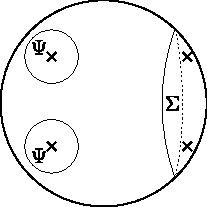
\includegraphics[width=0.3\linewidth]{V04_Psi2_Sigma.pdf}
  \caption{}
\end{figure}


A $\Sigma_n$ line of a diagram joins a $\Sigma_n$ slot of one vertex to a $\Sigma_n$ slot of another, and it carries $n$ strands, one per puncture of the slot.
Each strand is a sewing of two punctures through the inverse of the single-string pairing~\eqref{p:eq:hs1:pairing}, that is, the insertion of the level-matching bivector $b_0^- \delta_{L_0^-, 0}$ between them.
This is the sewing that produces the propagator of closed string field theory once the length of the plumbing cylinder is integrated with the insertion $b_0^+ / L_0^+$.
Here that insertion is absent: a strand is the plumbing at zero length, $w_1 w_2 = \e^{\I \theta}$, with only the twist $\theta$ integrated by the level-matching insertion, a legitimate CFT surface of measure zero in its moduli space.
A $\Psi$ line thus differs from a strand of a $\Sigma_2$ line by the integrated length alone, with its insertion $b_0^+ / L_0^+$, and not by the presence of an antighost, the level-matching insertion being common to both.
  This description holds for the pairing, and the line carries in addition the inverse $\sprod{2}{2}^{-1}$, which we discuss below.
A $\Sigma_2$ line is therefore not two strands of fixed length alone, and the surface picture of a diagram holds up to this factor.

The strands make a bookkeeping subtlety visible.
A chain of $k$ quartic vertices joined by $\Sigma_2$ lines is a tree when each line is counted as one edge, and the diagrams of \cref{p:sec:hs} are tree diagrams in this sense.
Their powers of $\gs$, their numbers of moduli and their ghost numbers are those of trees.
Resolved into punctures and strands, the same chain is the connected surface obtained by sewing $k$ spheres along $2 (k - 1)$ pairs of punctures, which has genus $k - 1$.
The two counts are reconciled by a formula that follows from the additivity of the Euler characteristic under sewing: a diagram with $L$ loops whose edges $e$ carry $k_e$ strands each has resolved genus
\begin{equation}
  \label{p:eq:ws:genus}
  g_{\mathrm{res}}
    = L + \sum_e (k_e - 1),
\end{equation}
so that a $\Sigma_2$ line raises the resolved genus by one and the loop number by zero.
No coupling and no modulus is attached to that genus, because the lengths of the necks that produce it are never integrated.
We can compare with a matrix model.
  There the double lines of a diagram fix the genus of its fat graph, and the expansion in $1 / N$ is an expansion in that genus.
  Here the strands also fix a genus, but no parameter counts it, and the physical expansion parameter $\gs$ organizes the diagrams by their loop number $L$, not by $g_{\mathrm{res}}$.

This suggests the structure of a colored operad, with one color per number of strands.
The objects are the spaces $\Hn{k}$ with their pairings $\pair[k]{\cdot}{\cdot}$.
The form $\sprod{2}{2}$ is a unary operation on the color $2$, and the cubic coupling $\vertex{4}(\Sigma_2, \Psi^2)$ is a corolla with one leg of color $2$ and two of color $1$.
Composition is the contraction of a $\Sigma_k$ line, an edge of color $k$, with the inverse of the $k$-string pairing.
The map that resolves a $\Sigma_2$ line into two ordinary strands is a linear map $\Hn{2} \hookrightarrow \Hs \otimes \Hs$ but not a map of operads, which is where the discrepancy in~\eqref{p:eq:ws:genus} comes from.
On the moduli-space side, the uncolored operad is the one of Kimura, Stasheff and Voronov on the decorated moduli spaces in which the vertex regions live~\cite{Kimura:1995:OperadStructuresModuli}.
We leave to future work the question whether the regions marked as above, together with a rule for the $\Sigma$ lines, form a colored operad of moduli spaces.
The obstacle is the line itself: its composition is not given by any kernel of the class defined below, and the one surface representation known, the Neumann series, carries algebraic factors.

